\chapter{ExxonMobil Model} 

The model utilizes a coupled axial-torsional system, considering the interactions between drill pipes, HWDP, collars, and other elements. By incorporating a lumped-parameter study, the model enables the investigation of the effects of various operating conditions on drill string behavior. Additionally, it integrates friction models, such as the consolidated friction model, to accurately represent the axial and tangential forces acting along the drill string, as well as the bit-rock interaction model (IADC/SPE-199678) to explain the cause of stick-slip. The validation of the model is achieved by comparing simulation results with field data from rotational startups, off-bottom rotations, and post-connection operations. 

The interaction between the bit and the rock is governed by a model based on the depth of cut. To incorporate Coulomb friction, the Stribeck friction model is employed, while borehole friction is considered through the use of viscous frictional forces. The net frictional force is influenced by factors such as gravity force, drilling mud properties, and well inclination. Reaction forces resulting from the bit-rock interaction occur when the bit is in contact with the formation. These forces persist for the duration that the bit remains on the bottom of the well. 


\subsection{Bit-rock Interaction}

A significant commonality observed in the aforementioned literature is the utilization of bit-rock interaction to explain the occurrence of stick slip. The laws governing the bit-rock interface in drilling operations primarily rely on the relationships between Weight on bit, torque on bit, rate of penetration, and angular velocity. These interdependent variables play a crucial role in achieving efficient drilling while also influencing the emergence of drilling dysfunctions within the system. The forces and torque exerted on the bit are directly influenced by the instantaneous changes in axial and angular velocities.

The interaction between PDC bits and the rock formation encompasses a combination of cutting and frictional contact, as identified by (Detournay and Defourny in 1992). Weight on bit and torque on bit are further decomposed into cutting and frictional components, which are contingent upon the strength of the rock formation being drilled.

\begin{equation}\label{WOB}
  WOB_{bit} = (k_{WOB}\times DOC_{iteration}) + (c_{bit-axial\times \dot{Z}_{bit-ietration}})
\end{equation}

\begin{equation}\label{Torque}
  TQ_{bit} = k_{TQ}\times DOC_{iteration\; array}\times (\pm1)
\end{equation}

where $k_WOB$, $k_TQ$ is Weight on bit and Torque coefficient, $DOC_iteration$ is depth of cut per iteration, $C_{bit-axial}$ is axial drag coefficient of bit and $Z$ is bit displacement 

The cutting components exhibit a direct dependency on the depth of cut, representing the material removed during drilling, while the frictional components are considered to account for the dissipated energy in the drilling process. To enhance the assessment of frictional forces at the bit and along the length of the drill string, particularly in deviated wellbores, a consolidated friction model (IADC/SPE-199678) is implemented within the drilling simulator. 


\subsection{Friction Model}

Modeling friction forces along the drill string is a challenging task due to the system's nonlinear behavior and the continuous changes in velocity direction. The net frictional force is highly influenced by the sliding velocity, with the axial component contributing to drag force and the tangential component generating frictional torque within the system.
 
%\begin{figure}
%  \centering
%  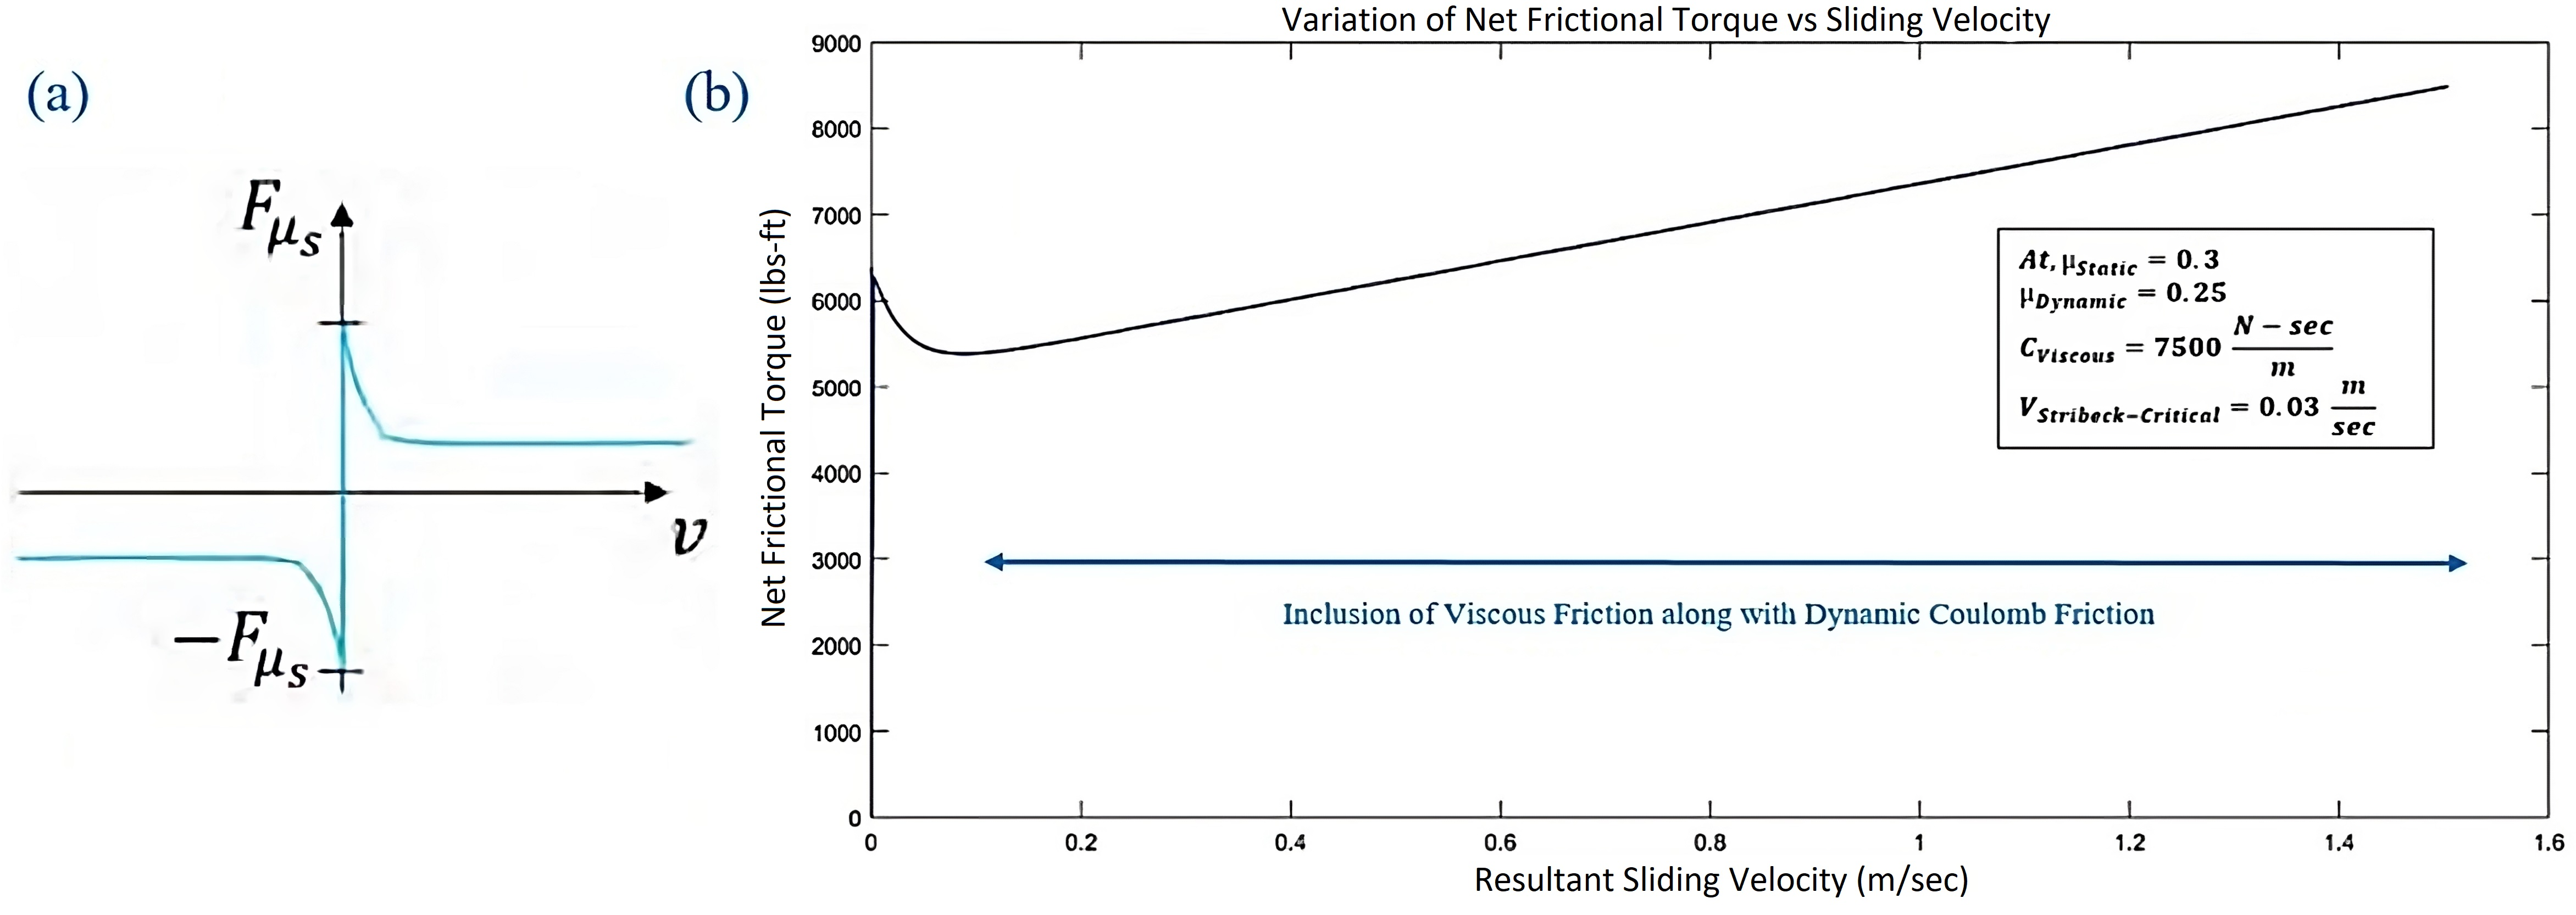
\includegraphics[width=4]{Stribeck}
%  \caption{Friction moedls: a) Wihtout Viscous Friction , b) Coulomb + Viscous Friction}\label{Friction models}
%\end{figure}

As the force of friction increases, it introduces a negative damping effect as the sliding velocity approaches zero. This negative damping effect can lead to stick-slip dysfunction, even when the bit is not in contact with the bottom of the well. In deviated wells, the axial velocity of the top drive and the drum's revolutions per minute do not instantaneously transfer to the bit. The elements of the drill string must overcome the static limits of friction to transfer energy to the next element. This lag in energy transfer is effectively described by the Stribeck curve, where the net frictional torque decreases as the sliding velocity increases.

\begin{equation}\label{dyanmic_force}
  F_{\mu\; k} = \mu_{k}\times F_{n} \times (Sign(V_{Sliding}))
\end{equation}

The dynamic friction force opposes the direction of axial motion, while static friction force $F_{\mu,s}$ acts in the opposite direction of the sum of all tangential forces when there is no sliding motion $V_{Sliding}=0$. The magnitude of the static friction force is equal to the sum of all tangential forces. This condition is valid when there is no sliding motion $V_{Sliding}=0$.

\begin{equation}\label{zero}
  F_{\mu,s} + \sum F_{Ext} = 0
\end{equation}

If, static friction calculated above is less than $\mu_{k}\times F_{n}$, where $\mu_{s} > \mu_{k}\times F_{n}$ then the surface is not sliding.

In order to avoid the discontinuities when $V_{iteration}$ tends to zero, Stribeck friction model is used. Following equation was proposed by Tustin 1947:

\begin{equation}\label{Stribeck velocity}
  F_{\mu,i} = F_{\mu_{k},i} + (F_{\mu_{s},i} - F_{\mu_{k},i})e^{-\dfrac{|\nu_{i}|}{\nu_{cs}}}
\end{equation} 

The model incorporates $F_{\mu,i}$ and $\nu_{CS}$ (Stribeck critical velocity) to consider the velocity weakening effect in the dynamics of the system. However, it should be noted that the model does not account for string Capstan effects.Furthermore, the order of the viscous damping constants is maintained consistently to ensure that the system remains in an ideal damp state, aligning with the field data. In the case of a multi-element string, the distribution of borehole dampers is considered by assigning damper values to each element based on the fraction of its mass contribution. For example, Collars are assigned 50\% of the damper value, HWDP is assigned 30\%, and drill-pipes are assigned 20\%. 

Below you will find the Friction model input parameters:

\begin{table}
  \centering
  \begin{tabular}{|m{3cm}|}
    \hline
    % after \\: \hline or \cline{col1-col2} \cline{col3-col4} ...
    Equivalent diameter of pipe\\
    \hline
    Coulomb Friction Force \\
    \hline
    Coulomb Friction Force Axial Component \\
    \hline
    Coulomb Friction Force Tangential Component \\
    \hline
    Coulomb Friction Torque Tangential Component \\
    \hline
    Viscous Friction Force Axial Component \\
    \hline
    Viscous Friction Force Tangential Direction Component \\
    \hline
    Axial and Tangential components of Net Frictional Force and Torque \\
    \hline
  \end{tabular}
  \caption{Input parameters for Friction model}\label{Table_Friction_Input}
\end{table}

\subsection{Governing equations and solution}

The set of partial differential equations that describe the motion of the drill-string can be combined into a coupled axial-torsional system of second-order differential equations. 

\begin{equation}\label{Governing equations}
  \begin{cases}
   \begin{aligned}
     m_{i}\dfrac{\partial^{2}s_{i}}{\partial t^{2}} & = -k_{a,i}(s_{i}-s_{i-1}-l_{i}) + k_{a,j+1}(s_{i+1}-s_{i}-l_{i+1}) + \sum{F_{ext, i}} \\
     I_{i}l_{i}\dfrac{\partial^{2}\theta_{i}}{\partial t^{2}} & = -k_{t,i}(\theta_{i}-\theta_{i-1}-l_{i}) + k_{t,j+1}(\theta_{i}-\theta_{i+1}) + \sum{\tau_{ext,/ i}}
   \end{aligned}
  \end{cases}
\end{equation}

To convert these equation sets into vector form, we can represent the variables and their derivatives as vectors.

\begin{equation}\label{Vector_form}
  \begin{aligned}
  & \{M\} \ddot{\boldsymbol{Z}}+\left\{C_a\right\} \dot{\boldsymbol{Z}}+\left\{K_a\right\} \boldsymbol{Z}+\boldsymbol{f}_{\text {fric }}=\boldsymbol{F}_{\text {forcing }} \\
  & \{J\} \ddot{\boldsymbol{\theta}}+\left\{C_t\right\} \dot{\boldsymbol{\theta}}+\left\{K_t\right\} \boldsymbol{\theta}+\boldsymbol{\tau}_{\text {fric }}=\boldsymbol{\tau}_{\text {forcing }}
  \end{aligne
\end{equation}


\begin{equation}\label{12}
  \begin{aligned}
  & \{M\}=\left[\begin{array}{ccc}
  m_1 & \cdots & \vdots \\
  \vdots & \ddots & \vdots \\
  \vdots & \cdots & m_n
  \end{array}\right] \\
  & \{J\}=\left[\begin{array}{ccc}
  J_1 & \cdots & \vdots \\
  \vdots & \ddots & \vdots \\
  \vdots & \cdots & J_n
  \end{array}\right] \\
  & \left\{C_a\right\}=\left[\begin{array}{ccc}
  c_{a 1} & \cdots & \vdots \\
  \vdots & \ddots & \vdots \\
  \vdots & \cdots & c_{a n}
  \end{array}\right] \\
  & \left\{C_t\right\}=\left[\begin{array}{ccc}
  c_{t 1} & \cdots & \vdots \\
  \vdots & \ddots & \vdots \\
  \vdots & \cdots & c_{t n}
  \end{array}\right] \\
  & \left\{K_a\right\}=\left[\begin{array}{ccc}
  k_{a 1} & -k_{a 2} & \cdots \\
  -k_{a 2} & \ddots & \vdots \\
  \vdots & \cdots & k_{a(n-1)}+k_{a n}
  \end{array}\right] \\
  & \left\{K_t\right\}=\left[\begin{array}{ccc}
  k_{t 1} & -k_{t 1} & \cdots \\
  -k_{t 1} & \ddots & \vdots \\
  \vdots & \cdots & k_{t(n-1)}+k_{t n}
  \end{array}\right] \\
  & F_{\text {forcing }}=\left[\begin{array}{c}
  \boldsymbol{k}_{a 1} \cdot Z_{\text {top\_drive}} \\
  \vdots \\
  -\boldsymbol{k}_{a\_\text{bit}} \cdot \text {DOC}
  \end{array}\right] \\
  & \mathcal{T}_{\text {forcing }}=\left[\begin{array}{c}
  \boldsymbol{k}_{t 1} \cdot \theta_{\text {top\_drive}} \\
  \vdots \\
  -\boldsymbol{k}_{t\_\text{bit}} \cdot \text {DOC}
  \end{array}\right]
  \end{aligned}
\end{equation}

Where:
\begin{itemize}
  \item $Z_o = \int V_0 , dt$ \\
  \item $m_n$: drill string element mass \\
  \item Z: bit position (downward direction considered as positive) \\
  \item $k_a$: axial stiffness of drill-string element \\
  \item $V_o$: Top-drive (draw-works) axial velocity as input \\
  \item $Z_{top\_drive}$: Top-drive (draw-works) axial displacement as input \\
  \item $\dot{Z}$: bit axial velocity (downward direction considered as positive) \\
  \item $WOB_{\text{Surface}}$: Surface/Top-drive WOB (In ROP Control Mode) \\
  \item $J_n$: mass moment of inertia of drill string element \\
  \item $\theta$: \text{rotation angle (Clockwise direction is considered as positive)} \\
  \item $\omega_o$: Topdrive angular velocity as input \\
  \item $\theta_{top\_drive}$: Topdrive rotation as input \\
  \item $k_t$: Torsional stiffness of drill-string \\
  \item $\dot{\theta}$: bit rotary velocity (Clockwise direction considered as positive) \\
  \item $TQ_{\text{Surface}}$: Surface/Top-drive Torque \\
\end{itemize}


The differential equation sets are solved using the ODE45 solver. ODE45 is a versatile numerical solver that employs the Runge-Kutta method with a variable time step. This solver is chosen for its efficiency in computational calculations.

